%##########################################################################
%                                                                     
%                         Care-O-bot Manual                                                        
%                                     
%##########################################################################


%##########################################################################
% Formatierungsoptionen
% fuer Bilder die Option "draft" entfernen
\documentclass[12pt,twoside]{report}

% Standard Style-Files
%\usepackage{german}
\usepackage{a4}
%\usepackage{psfig}
\usepackage{graphicx}
\usepackage{subfigure}
%\usepackage{equations}
\usepackage{thb}
\usepackage{amssymb}
\usepackage{listings}

% define colors
\usepackage{color}
\definecolor{light-gray}{gray}{0.85}

% Abruerzungsverzeichnis
\usepackage{nomencl}

% Hyperlinks
\usepackage[bookmarksnumbered=true,backref=page,breaklinks=true,pdftitle={Care-O-bot manual},
pdfauthor={Nadia Hammoudeh Garcia, Florian Weisshardt},pdfsubject={Care-O-bot administration and user manual},
pdfkeywords={Care-O-bot, ROS, setup, install, manual}]{hyperref}


% Seitenstil
\pagestyle{headings}
%
% Abstand zwischen Abs"atzen
\setlength{\parskip}{1.5ex}

% Einr"uckung der ersten Zeile eines Absatzes unterdr"ucken
\setlength{\parindent}{0pt}

% Grosszuegigere Wortabstaende
\sloppy

% Tiefe der numerierten Kapitel definieren
\setcounter{secnumdepth}{3}

% Tiefe der Kapitel im Inahltsverzeichnis definieren
\setcounter{tocdepth}{2}


% Damit Bilder m"oglichst da sind, wo man sie will
\setcounter{topnumber}{20}
\setcounter{bottomnumber}{20}
\setcounter{totalnumber}{20}
\renewcommand{\topfraction}{.9999}
\renewcommand{\bottomfraction}{.9999}
\renewcommand{\textfraction}{0}

% source code
\lstset{
basicstyle=\footnotesize,
frame=single,
breaklines=true,
backgroundcolor=\color{light-gray}
}


%##########################################################################
% Abkuerzungen 
\let\abbrev\nomenclature
\renewcommand{\nomname}{Abk"urzungsverzeichnis} 
\setlength{\nomlabelwidth}{.24\hsize} % Punkte zw. Abkrzung und Erklrung
\renewcommand{\nomlabel}[1]{#1 \dotfill}
%\setlength{\nomitemsep}{-\parsep} % Zeilenabstnde verkleinern
\makenomenclature 
% einfuegen mit \abbrev{Abkuerzung}{Beschreibung}


%###########################################################################
% Bearbeitung von einzelnen Kapiteln

%\includeonly{berichttitle}
%\includeonly{berichttoc}
%\includeonly{bericht1}
%\includeonly{bericht2}
%\includeonly{bericht3}
%\includeonly{bericht4}
%\includeonly{bericht5}
%\includeonly{berichtapp}
%\includeonly{berichtlof}
%\includeonly{berichtloc}
%\includeonly{berichtlot}
%\includeonly{berichtbib}


%###########################################################################
\begin{document}

% Titelseite einfgen
%###########################################################################
%
%   Titelseite
%
%###########################################################################
\begin{titlepage}
\vspace*{13mm}
\begin{center}
  \vspace{10mm} 
         {\large \hspace{20mm} Care-O-bot Manual\\}
  \vspace{10mm}
       {\Large
          \bf
          \hspace{20mm} Manual for Care-O-bot users\\} 
  \vspace{5mm}
       {\Large
          \bf
          \hspace{20mm} and administrators\\}

  \vspace{80mm}
  \makebox[40mm]{\large \hspace{16mm} Autors: }\makebox[65mm][l]
                                   {\large Florian Weisshardt}
  \makebox[40mm]{}\makebox[65mm][l]{\large Nadia Hammoudeh Garcia}\\
% \makebox[40mm]{}\makebox[65mm][l]{\large Name}\\
  \vspace{10mm}
         {\large \hspace{20mm} Fraunhofer IPA} \\
  \vspace{5mm}
         {\large \hspace{20mm} Institute for Manufacturing Engineering and Automation} \\
         {\large \hspace{20mm} Stuttgart, Germany} \\
  %\vspace{20mm}
  \vfill
         {\large \hspace{20mm} Last modified on \today}
\end{center}
\end{titlepage}

\clearpage
\thispagestyle{empty}
\cleardoublepage
\thispagestyle{empty}\cleardoublepage % Inhalt auf der rechten Seite beginnen

% Raendereinstellungen fuer Doppelseitigen Ausdruck
\evensidemargin=2pt
\oddsidemargin=40pt

% Zeilenabstand strecken
\renewcommand{\baselinestretch}{1.15}\normalsize


\pagenumbering{roman}

% Inhaltsverzeichnis einfgen
\tableofcontents
\thispagestyle{empty}\cleardoublepage

% Abkrzungsverzeichnis einfgen
%\include{berichtnom}
%\thispagestyle{empty}\cleardoublepage

% Kapitel einfgen
\pagenumbering{arabic}
\chapter{Introduction}
\label{chap:introduction} 

This manual is divided into three main parts. The first part (chapter \ref{chap:user}) is intended for all users, it shows how to startup the robot, login and execute simple commands on the robot. The second part (chapter \ref{chap:admin}) addresses robot administrators and covers topics like setting up the pcs, configuring network and add new user accounts. The third part (chapter \ref{chap:support}) offers some first help in case you need support.

You can always get the latest version of this manual at \footnote{\url{https://github.com/ipa320/setup/blob/master/manual/Care-O-bot_manual.pdf}}.

If you have comments, suggestions or would like to add something to the manual, please contact \href{mailto:fmw@ipa.fhg.de}{fmw@ipa.fhg.de}.
\chapter{User Manual}
\label{chap:user}    

{\colorbox{red}{\textbf{NOTE:}}}\textbf{ Before you start working with the robot you have to attend a safety introduction. If you haven't got one yet, please contact your local robot administrator.}

\section{Hardware overview}
You can take a look of the technical data of Care-O-Bot on the official web site\footnote{\url{http://www.care-o-bot-research.org/care-o-bot-3/technical-data}} and \footnote{\url{http://www.care-o-bot-research.org/care-o-bot-3/components}}. Also you can see the distribution of the different Care-O-bots at \footnote{\url{http://www.ros.org/wiki/Robots/Care-O-bot/distribution}}.

An overview of the robot hardware is shown in the following picture.
\begin{center}
 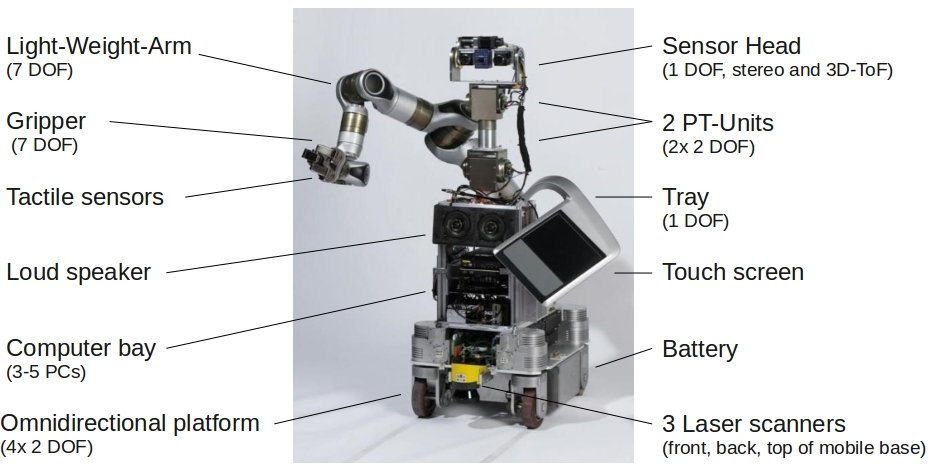
\includegraphics[width=0.95\textwidth]{images/hardware_overview.jpg}
\end{center}

\section{Software overview}\label{sec:software_overview}
We defined a layer called \textit{bringup layer}, which covers all hardware drivers and basic robot components. This is the layer where low level robot movements are enabled through the joystick or dashboard and the robot status including actuator and sensor information is acquired. In the following overview you can see the repositories which belong to the bringup layer.
\begin{itemize}
\item \texttt{cob\_extern}: The \texttt{cob\_extern} stack contains third party libraries needed for operating Care-O-bot. The packages are downloaded from the manufacturers website and not changed in any way.
\item \texttt{cob\_common}: The \texttt{cob\_common} stack hosts common packages that are used within the Care-O-bot repository. Also the urdf description of the robot, which is the kinematic and dynamic model of the robot, 3D models of robot components, information required for gazebo to simulate the COB and utility packages or common message and service definitions.
\item \texttt{schunk\_modular\_robotics}: This repository includes drivers and models for Schunk products, like powercubes or sdh.
\item \texttt{cob\_driver}: The cob\_driver stack includes packages that provide access to the Care-O-bot hardware through ROS messages, services and actions. E.g. for mobile base, arm, camera sensors, laser scanners, etc...
\item \texttt{cob\_command\_tools}: This stack provides the source code of the tools that you need to command the robot: \texttt{cob\_command\_gui}, \texttt{cob\_dashboard}, \texttt{cob\_script\_server} and \texttt{cob\_teleop}.
\item \texttt{cob\_robots}:  The \texttt{cob\_robots} stack collects Care-O-bot components that are used in bringing up a robot. The user's interface to the \texttt{cob\_robots} stack is \texttt{cob\_bringup}. In this package you find all the hardware configuration and launch files to bringup the hardware.
\item \texttt{cob\_environments}: This stack provides the parameters for default environment configurations.
\end{itemize}

\section{Batteries and power supply}
Care-O-bot is powered by a 48V battery, which can be a Gaia rechargeable Li ion battery (60 Ah 48V) or a plumb battery. The batteries can be charged with a maximum of 56V at 10A. The robot can be plugged in during operation.

\section{Emergency stop}\label{sec:emergency_stop}
Please be aware that not all robot movements are safe for you as an user, the robot itself and the environment. Therefore please don't hesitate to activate the emergency stop in situations which are not foreseen by the user. There are three ways of stopping the robot: On the robot you have two red buttons on the laterals, you can step into the safety fields of the Sick S300 scanners or you use the wireless emergency stop. Remember to recover the robot components with the command\_gui after an emergency stop was activated, check the status of the components using the dashboard.

\subsection{Emergency stop buttons}
Press the red buttons on the left and right side of the torso. To release the emergency stop, turn the buttons so that they come out again. After that turn the key to position II until you hear a "click".

\begin{center}
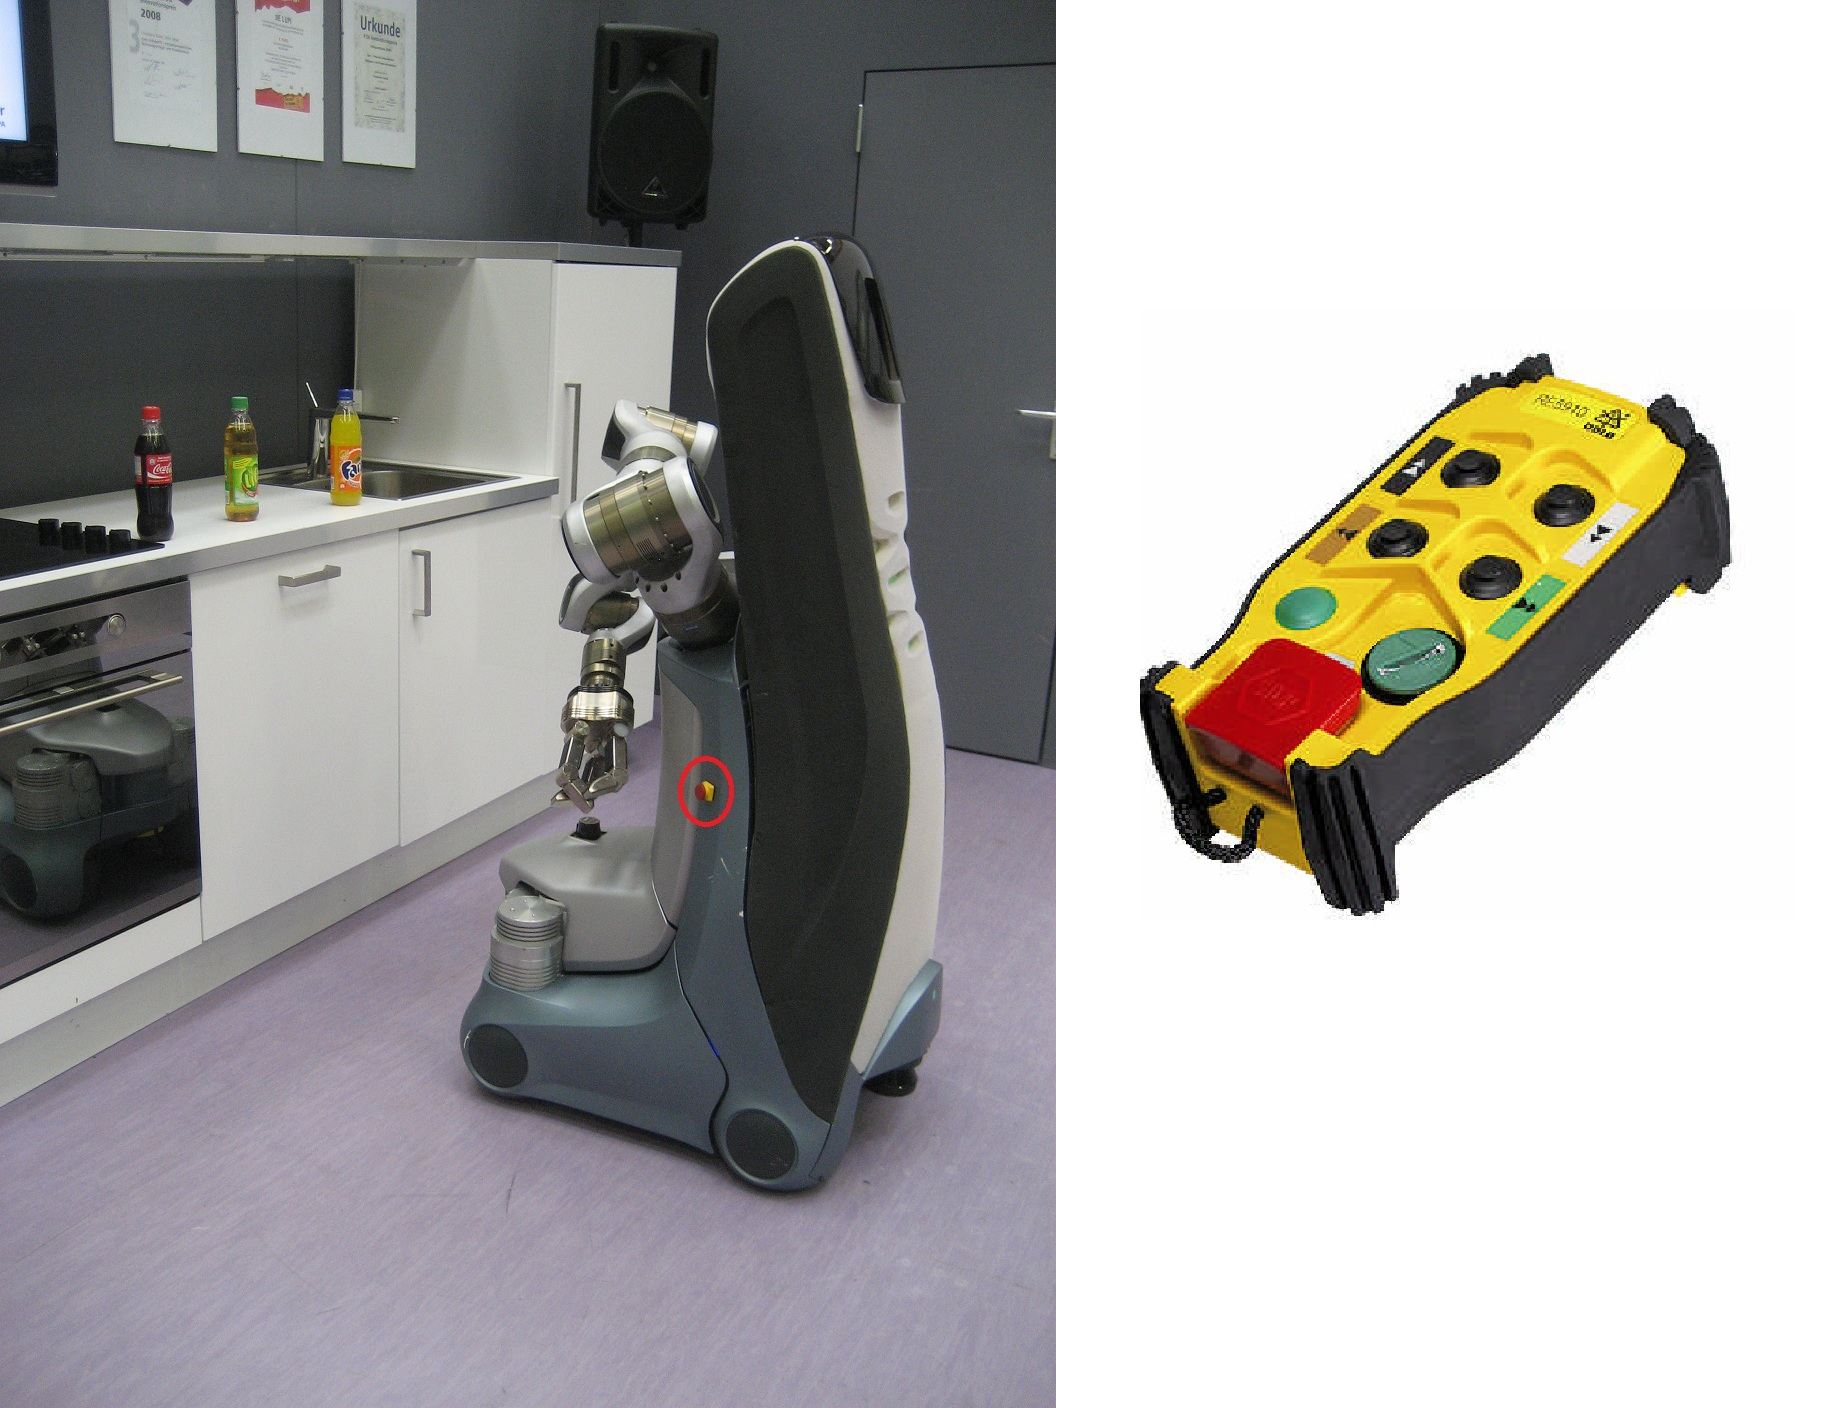
\includegraphics[width=0.65\textwidth]{images/em_stop.jpg}
\end{center}

\subsection{Safety field from the Sick S300 scanners}
If you step into the safety fields of the laser scanners the emergency stop is activated automatically. After the safety fields are free from any obstacle again the emergency stop is released on its own after a few seconds.

\begin{center}
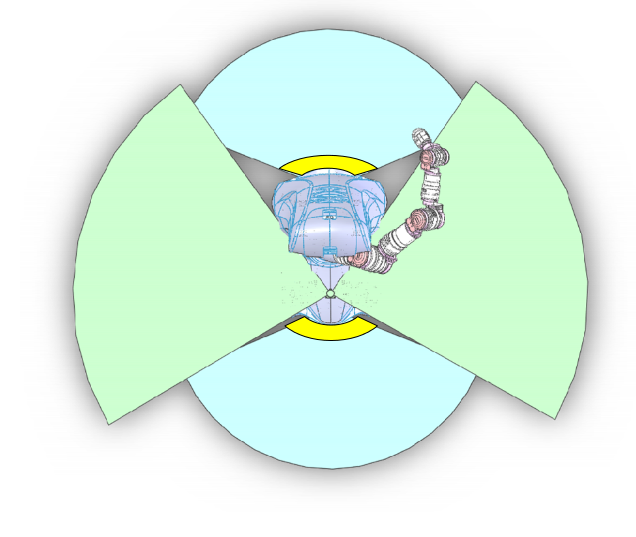
\includegraphics[width=0.65\textwidth]{images/protection_areas.png}
\end{center}

\subsection{Remote emergency stop control}
You can press the red button to stop the robot. To release the emergency stop you have to lift the red button and afterwards press the green button.


\textbf{NOTE}: If you hear a "click" while releasing the emergency stop, but the dashboard and command\_gui still show that the emergency stop is activated, turn the key to position II again and hold it for some seconds until the dashboard or command\_gui show no more emergency stop.


\section{Running the robot}
First you have to connect the power supply to the robot or you can use the battery pressing the battery button on the base. To switch the robot on you have to use the key. If you move it to position II and hold for a few seconds the robot will turn on. To turn of the robot turn the key to position I. 

After starting up the robot the emergency stop circuit is still activated. To enable power for the motors, keep the safety area of the Sick S300 scanners free of any obstacle and release the emergency buttons. In the case that the wireless emergency stop is active, release it by releasing the red button and pressing the green button afterwards. You should hear a "click" as soon as the emergency stop is released.

For safety reasons if the robot is not supervised any more, e.g. during a break, the emergency stop has to be activated. Never operate the robot without a local person supervising it being aware of the safety instructions (see separate safety instructions).

\begin{center}
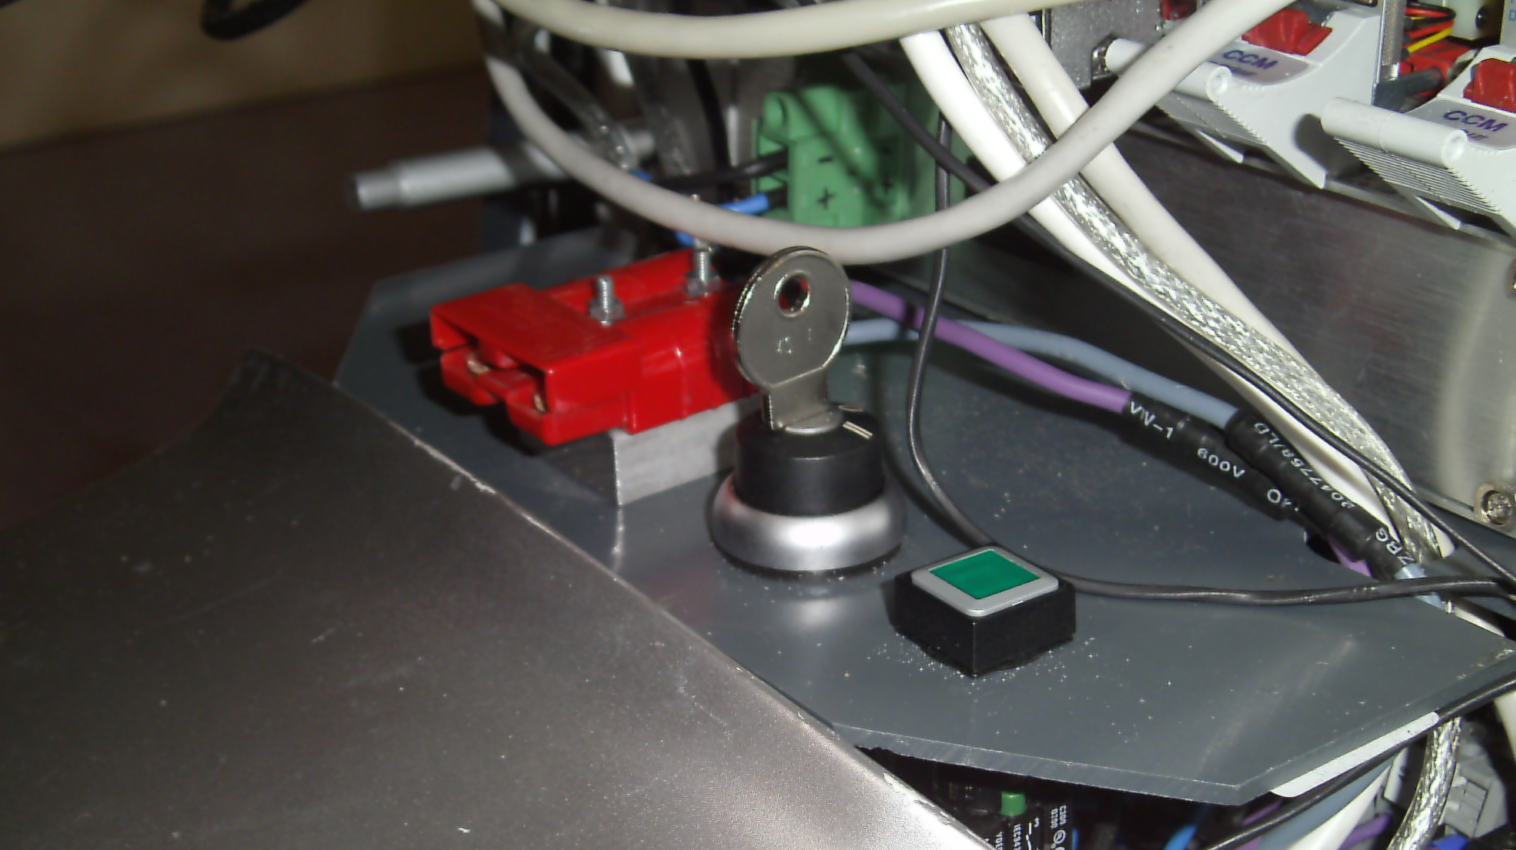
\includegraphics[width=0.3\textwidth]{images/key.png}
\end{center}


\subsection{Logging in to the robot pcs}
For logging in with a remote PC to the robot pcs you have to have an account on the robot. If you don't have an account contact your local robot administrator to create one for you (see the section \ref{sec:account}). Use ssh to login (in this example to pc1 of cob3-3)

\begin{lstlisting}
ssh -X user_name@cob3-3-pc1
\end{lstlisting}

\subsection{Bringup the robot}
\textbf{Note: The following steps can only be done once by one person at the same time. It is not possible to start for example mulitple roscore or brinup.}

The first step to bringup the robot is to start a roscore, this is necessary to have communication between the nodes. You can run it using
\begin{lstlisting}
roscore
\end{lstlisting}

If you want to run the robot you have a launch file for launching all the components of the robot. It is located in the package cob\_bringup.
\begin{lstlisting}
roslaunch cob_bringup robot.launch
\end{lstlisting}

Now all drivers and core components should be started so you can continue and have a look at the robot status in the dashboard or moving the robot using joystick or command\_gui.

\subsection{Using dashboard and command\_gui}
To know the state of all the components of the robot you can use the dashboard tool. To move the robot you can use the command\_gui. You can start both with
\begin{lstlisting}
roslaunch cob_bringup dashboard.launch
\end{lstlisting}

After launching this file you will see two GUIs on your screen: the smaller one is the dashboard, which gives you information about the current status of the robot and its components as well as the emergency stop status. The bigger one is called command\_gui and offers a wide range of buttons to move the robot to predefined positions using low level control commands. It also offers buttons for initialising and recovering the actuators. The emergency stop status is visible in the upper left corner of the command\_gui. Before initialising or moving the robot, check that the status is OK.

\subsubsection{cob\_dashboard}\label{subsec:dashboard}
The dashboard is an important tool where you can check the state of the robot, it is recommended that you have it always opened. The dashboard looks like this:

\begin{center}
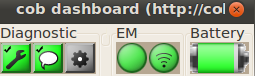
\includegraphics[width=0.55\textwidth]{images/dashboard.png}
\end{center}
If you click the first button, you will see a new window popping up with three levels: Errors, Warnings and All. There you can see the state of each component at any time. The status monitoring is divided into Actuators, Sensors and other. The other buttons are for showing diagnostics, motors, emergency status and battery state. In the case of the Care-O-bot we have disable the buttons for the Motors, you see them always in red.

\begin{center}
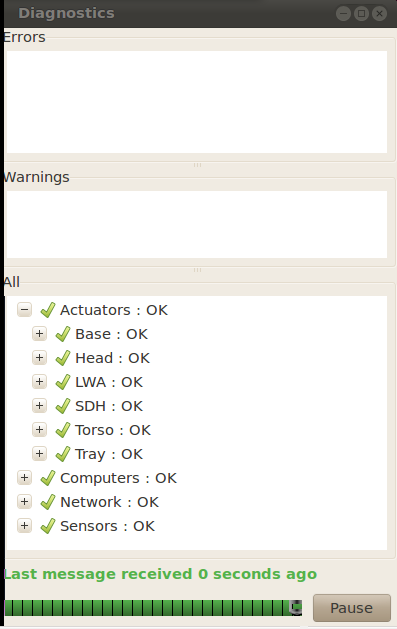
\includegraphics[width=0.45\textwidth]{images/diagnostics.png}
\end{center}

All diagnostics information for the actors and sensors should be green after successfully initializing the components, see section \ref{subsec:command_gui}.

\subsubsection{cob\_command\_gui}\label{subsec:command_gui}
The command gui can be used for sending low level movement commands to the robot components. The standard view of the command\_gui is:
\begin{center}
 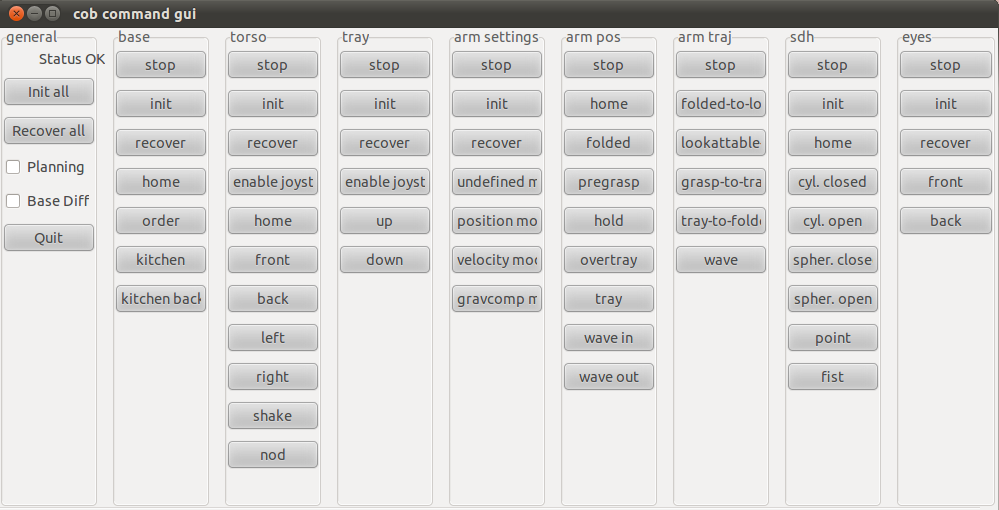
\includegraphics[width=1\textwidth]{images/cob_command_gui.png}
\end{center}

In this screen-shot you can see different columns: general, base, torso, tray, arm settings, arm pos, arm traj, sdh and eyes. The first column is very important, when you run the robot. If you want to move it, first initialize all components with a click on \texttt{init all} and make sure that the \textbf{emergency stop is not active}. It will take some time and the actuators will do their homing sequence if necessary. After an emergency stop was activated, each component has to be recovered. Therefore press the button \texttt{recover all}. 

The other columns of the components have different predefined positions where you can move to. Additionally Each component has a \texttt{stop}, \texttt{init} and \texttt{recover} button, to stop, initialize or recover a single component.

\subsection{Rviz}
RVIZ is a tool that visualizes data from the robot, e.g. the sensor data from the laser scanners, but also information about the coordinate systems and transformations or the images from the cameras. You can add your own items to RVIZ to visualize topics, see more information at \footnote{\url{http://www.ros.org/wiki/rviz}}.

RVIZ needs to be started on your local machine. To be able to visualize topics from the robot export your \texttt{ROS\_MASTER\_URI} to the robot
\begin{lstlisting}
export ROS_MASTER_URI=http://cob3-X-pc1:11311
rosrun rviz rviz
\end{lstlisting}

To use a predefined configuration for Care-O-bot start rviz with
\begin{lstlisting}
export ROS_MASTER_URI=http://cob3-X-pc1:11311
roslaunch cob_bringup rviz.launch
\end{lstlisting}

You will see a screen like this:
\begin {center}
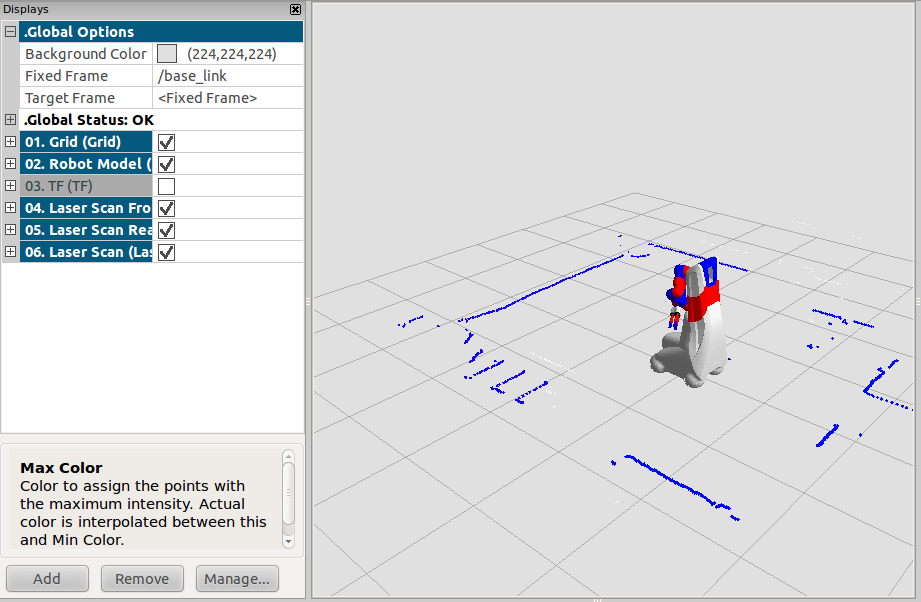
\includegraphics[width=1\textwidth]{images/rviz.png}
\end{center}

\subsection{Joystick}
To be able to use the joystick, initialize the components using the command\_gui. For moving the robot components, the dead-man\_button has to be pressed all the time, as soon as the button is released all hardware components will be stopped immediately. 

\begin{itemize}
\item For moving the base: Hold the dead-man button and use the base rotation and translation axis to move the base.
\item For moving the torso: Hold the dead-man button and the upper or lower neck button, then use the up\_down or left\_right axis to move the torso.
\item For moving the tray: Hold the dead-man button and the tray button, then use the up\_down axis to move the tray.
\item For moving the arm: Hold the dead-man button and one of the arm buttons, then use the up\_down or left\_right axis to move the selected arm joints.
\end{itemize}

Have a look at the following image to see which buttons command which components. 
\begin{center}
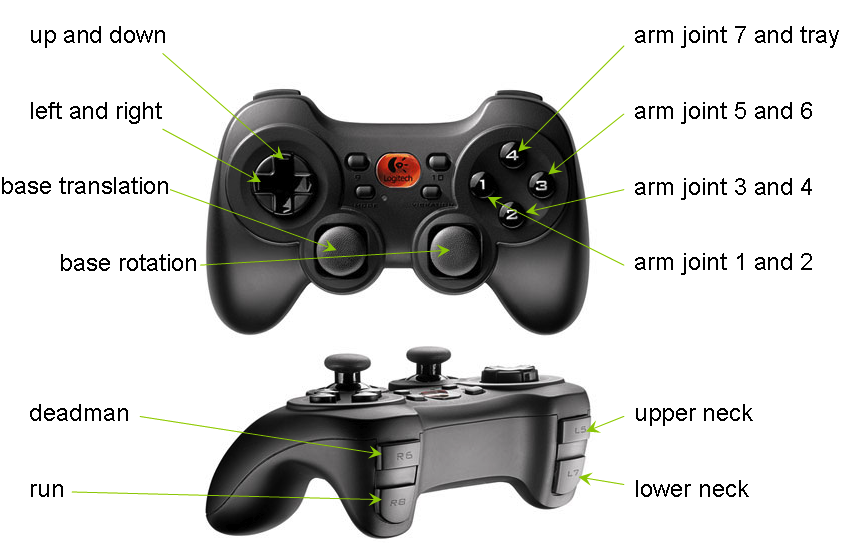
\includegraphics[width=1\textwidth]{images/joystick.png}
\end{center}

\section{Power down the robot}
To power down the robot turn the key to position I, disconnect the power cable and turn off the power supply.

\section{Packing the robot}
tbd
\chapter{Administrator manual}
\label{chap:admin}

%#################################################################################################
\section{Setup robot pcs}
%#################################################################################################
On all Care-O-bots there are at least two pcs. Some Care-O-bots have an optional third pc, which is not coveres by this manual. Within this section we will guide you through setting up new pcs. When nothing otherwise is mentioned the following instructions are for both pc1 and pc2, please do the same steps on both pcs.

To pc1 all actuators are connected, sensors are connected both, to pc1 and pc2. All camera sensors are connected to pc2, whereas all other sensors like e.g. laser scanners are connected to pc1. By default pc3 is not connected to any hardware and therefore can be used as additional computing power.

\subsection{Install operating system}
The first step is to install the operating system for each pc, which means pc1 and pc2 (optionally pc3). We are using Ubuntu as the main operating system for the robot. We recommend to install the \textbf{Ubuntu 10.4 LTS (long term stable) 64-bit} version because this version is well tested to work with the hardware. 

For the first installating please install Ubuntu (english version) creating a normal swap partition. Please choose \textit{robot} as an admin account with a really safe password which should only be known to the local robot administrator. The hostname of the pc should be \textit{cob3-X-pc1} and \textit{cob3-X-pc2}.

\subsection{Install basic tools}
Next we have to install some basic tools for the further setup of the pcs. In order to install the packages a internet connection is needed.

\begin{lstlisting}
sudo apt-get update
sudo apt-get install vim tree openssh-server gitg meld curl
\end{lstlisting}

To facilitate the further setup we created a setup repository with some helpfull scripts. To checkout the setup repository use:

\begin{lstlisting}
mkdir ~/git
cd ~/git
git clone git://github.com/ipa320/setup.git
\end{lstlisting}

\subsection{Setup internal robot network}
Inside the robot there's a router which connects the pcs and acts as gateway to the building network. Setup the router with the following configuration. 

The ip adress of the router should be \textbf{192.168.0.1} and for the internal network dhcp should be activated. Use \textbf{cob3-X} as hostname for the router. Register the MAC adresses of pc1 and pc2 so that they get a fixed ip adress over dhcp. Use \textbf{192.168.0.101 for pc1} and \textbf{192.168.0.102 for pc2}. Enable \textbf{portforwarding} for port 2201 to 192.168.0.101 and for port 2202 to 192.168.0.102.

After ensuring that the network configuration of the router is setup correctly, we can configure the pcs. All pcs should have two ethernet ports. The upper one should be connected to the internal router. Sometimes the graphical network manager causes troubles, so it is best to remove it

\begin{lstlisting}
sudo apt-get remove network-manager
\end{lstlisting}

After removing the network manager we will have to edit \textit{/etc/network/interfaces} manually. 

\subsubsection{Network configuration on pc1}

\begin{lstlisting}
auto lo
iface lo inet loopback

auto eth0
iface eth0 inet static
address 192.168.0.101 # internal ip adress of pc1
netmask 255.255.255.0 # netmask

auto eth1
iface eth1 inet static
address 192.168.42.1 # ip adress for controller network
netmask 255.255.255.0 # netmask
\end{lstlisting}

\subsubsection{Network configuration on pc2}

\begin{lstlisting} 
auto lo
iface lo inet loopback

auto eth0
iface eth0 inet static
address 192.168.0.102 # internal ip adress of pc2
netmask 255.255.255.0 # netmask

auto eth1
iface eth1 inet static
address 192.168.21.99 # ip adress for camera network
netmask 255.255.255.0 # netmask
\end{lstlisting}

\subsection{Install NFS}
After the network is configured properly we can setup a NFS netween the robot pcs. pc2 will act as the NFS server and pc1 as NFS client.

\subsubsection{NFS configuration on pc2 (server)}
Install the NFS server package and create the NFS directory

\begin{lstlisting}
sudo apt-get install nfs-kernel-server
sudo mkdir /u 
\end{lstlisting}

Add the following following line to \textit{/etc/fstab}:

\begin{lstlisting}
/home	/u	none	bind	0	0
\end{lstlisting}

Now we can mount the drive

\begin{lstlisting}
sudo mount /u
\end{lstlisting}

Activate IDMAPD in \textit{/etc/default/nfs-common} by changing the NEED\_IDMAPD to yes

\begin{lstlisting}
NEED_IDMAPD=yes
\end{lstlisting}

Copy the file \textit{$\sim$/git/setup/nfs\_setup/server/exports} to \textit{/etc/exports}

\begin{lstlisting}
cp ~/git/setup/nfs_setup/server/exports /etc/exports
\end{lstlisting}

Change the home directory of the \textit{robot} user from \textit{/home/username} to \textit{/u/username} in the \textit{/etc/passwd} file.

After finishing you need to reboot the pc

\begin{lstlisting}
sudo reboot
\end{lstlisting}

\subsubsection{NFS configuration on pc1 (client)}
Install the NFS client package and create the NFS directory

\begin{lstlisting}
sudo apt-get install nfs-kernel-server autofs
sudo mkdir /u
\end{lstlisting}

Activate IDMAPD in \textit{/etc/default/nfs-common} by changing the NEED\_IDMAPD to yes

\begin{lstlisting} 
NEED_IDMAPD=yes
\end{lstlisting}

Edit \textit{/etc/auto.master} and add

\begin{lstlisting}
/-	/etc/auto.direct
\end{lstlisting}

Copy the file \textit{$\sim$/git/setup/nfs\_setup/client/auto.direct} to \textit{/etc/auto.direct}

\begin{lstlisting}
cp ~/git/setup/nfs_setup/client/auto.direct /etc/auto.direct
\end{lstlisting}

Activate the NFS

\begin{lstlisting}
sudo update-rc.d autofs defaults
sudo service autofs restart
sudo modprobe nfs
\end{lstlisting}

Change the home directory of the \textit{robot} user from \textit{/home/username} to \textit{/u/username} in the \textit{/etc/passwd} file.

After finishing you need to reboot the pc

\begin{lstlisting} 
sudo reboot
\end{lstlisting}

\subsection{Setup NTP time synchronitation}
Install the ntp package

\begin{lstlisting}
sudo apt-get install ntp
\end{lstlisting}

\subsubsection{NTP configuration on pc1 (NTP server)}
Edit \textit{/etc/ntp.conf}, change the server to \textit{0.pool.ntp.org} and add the restrict line

\begin{lstlisting} 
server 0.pool.ntp.org
restrict 192.168.0.0 mask 255.255.255.0 nomodify notrap
\end{lstlisting}

\subsubsection{NTP configuration on pc2 (NTP client)}
Edit \textit{/etc/ntp.conf}, change the server to \textit{cob3-X-pc1}:
\begin{lstlisting}
server cob3-X-pc1
\end{lstlisting}

\subsection{Install ROS and Care-O-bot driver software}
For general instructions see \url{http://www.ros.org/wiki/Robots/Care-O-bot/electric}.

\subsubsection{Install ROS and additional tools}
\begin{lstlisting}
sudo apt-get install openjdk-6-jdk zsh terminator
sudo apt-get install python-setuptools
sudo easy_install -U rosinstall
sudo apt-get install ros-diamondback-care-o-bot ros-diamondback-perception-pcl-addons ros-diamondback-erratic-robot
sudo apt-get install ros-electric-care-o-bot ros-electric-perception-pcl-addons ros-electric-pr2-desktop ros-electric-pr2-robot ros-electric-pr2-apps pr2-power-drivers 
\end{lstlisting}

\subsubsection{Setup bash environment}
We setup a special bash environment to be used on the Care-O-bot pcs. The environments differ from pc1, pc2 and pc3. Copy the \textit{cob-bash-bashrc.pcX} to \textit{/etc/cob-bash-bashrc} on each pc.

\begin{lstlisting}
sudo cp ~/git/setup/cob-pcs/cob-bash-bashrc.pcX /etc/cob-bash-bashrc
\end{lstlisting}

All users have a pre-configured bash environment too, therefore copy \textit{user.bashrc} to \textit{$\sim$/.bashrc}
\begin{lstlisting}
cp ~/git/setup/cob-pcs/user.bashrc ~/.bashrc
\end{lstlisting}

If you logout and login again or source your \textit{$\sim$/.bashrc}, you should see different terminal colors for each pc and the \textit{ROS\_PACKAGE\_PATH} should be configured. If you check 
\begin{lstlisting}
roscd cob_bringup
\end{lstlisting}
you should end up in \textit{/u/robot/git/care-o-bot/cob\_robots/cob\_bringup}

\subsubsection{Setup hardware components}
In order to use the different hardware components we have to install the drivers and set permission rights. All hardware configuration is stored in the \textit{cob\_hardware\_config} package.

\paragraph{Setup udev rules}
TIn order to have fixed device names we setup udev rules for Care-O-bot. Copy the udev rules from the setup repository to \textit{/etc/udev/rules.d} on pc1:
\begin{lstlisting}
sudo cp ~/git/setup/udev_rules/01-cob.rules /etc/udev/rules.d
\end{lstlisting}

\paragraph{Sick S300 laser scanners}
The Sick S300 scanners on the frontside and backside of the robot are connected via USB to pc1. To recevice data from the Sick S300 scanners check if the user is in the \textit{dialout} group
\begin{lstlisting}
groups
\end{lstlisting}

For testing you can run the front laser scanner with
\begin{lstlisting}
roslaunch cob_bringup laser_front.launch
\end{lstlisting}

To check if there is some data published use
\begin{lstlisting}
rostopic hz /scan_front
\end{lstlisting}

Check the rear scanner in the same way.

tbd, setup safety region

\paragraph{Hokuyo URG laser scanner}
tbd

\paragraph{Relayboard}
tbd

\paragraph{Base}
tbd, configure elmo controllers

\paragraph{Tray sensors}
tbd, phidget

\paragraph{Schunk SDH with tactile sensors}
tbd, firmware version
Add the robot user to the group dialout in the /etc/group file.

\paragraph{Schunk powercubes}
tbd, pcan

\paragraph{Head axis}
tbd

\paragraph{Prosilica cameras}
You have to define the ip address for the cameras, on pc2 in the file /etc/network/interfaces you can copy these lines:
\begin{lstlisting}
auto eth1 
iface eth1 inet static
address 192.168.21.99   # IP of network adapter to cameras 
netmask 255.255.255.0   # netmask
\end{lstlisting}

\paragraph{Kinect}
pc2


\subsection{Create a new user account}
\label{sec:account}
Due to the fact that all users need to be in the correct user groups, that the bash environment needs to be setup correctly and that user ids need to be synchronised between all pcs for the NFS to work, we facilitate the creation of a new user with a \textit{cobadduser} script. Before you add the first user using the \textit{cobadduser} script, please uncomment the following two lines in \textit{/etc/adduser.conf} on pc2
\begin{lstlisting}
EXTRA_GROUPS="dialout cdrom floppy audio video plugdev users"
ADD_EXTRA_GROUPS=1
\end{lstlisting}

After that you can add a new user. On pc2 and with administration rights you can use the following instruction
\begin{lstlisting}
cd ~/git/setup
sudo ./cobadduser new_user_name
\end{lstlisting}

All you need to do now is to login as the new user, create an ssh-key and add the key to the authorized keys to be able to login to all pcs without password. This is neccesarry for launching nodes remotely on all pcs.
\begin{lstlisting}
ssh-keygen
ssh-copy-id cob3-X-pc1
\end{lstlisting}


\section{Network}
Make sure you have name resolution and access to the robot pcs from your external pc. To satisfy the ROS communication you need a full DNS name lockup for all machines. Check it from your remote pc with
\begin{lstlisting}
ping 192.168.0.101
ping cob3-X-pc1
\end{lstlisting}
and the other way round try to ping your remote pc from one of the robot pcs
\begin{lstlisting}
ping your_ip_adress
ping your_hostname
\end{lstlisting}

If ping and DNS is not setup correctly, there are multiple ways to enable access and name resolution.

\subsection{Setting up your building network}
Setting up you building network to enable dns and portforwarding to the internal network.

\subsection{Manual setup for each remote pc}
You can setup a route to the internal network addresses. Please change the robot name and your network device to fit your settings. E.g. for connecting to cob3-X on eth0
\begin{lstlisting}
sudo route add -net 192.168.0.0 netmask 255.255.0.0 gw cob3-X dev eth0
\end{lstlisting}

for connecting to cob3-X on wlan0
\begin{lstlisting}
sudo route add -net 192.168.0.0 netmask 255.255.0.0 gw cob3-X dev wlan0
\end{lstlisting}


For name resolution you will probably have to edit the file \textit{/etc/hosts} on the robot pcs as well as on the remote pc. Therefore add the following addresses to the \textit{/etc/hosts} of your remote pc.
\begin{lstlisting}
192.168.0.101 cob3-X-pc1
192.168.0.102 cob3-X-pc2
192.168.0.103 cob3-X-pc3
\end{lstlisting}

Add your ip adress and hostname to the \textit{/etc/hosts} of all robot pcs.

\section{Calibration}
Now is not working....
\section{Backup and restoring users}   
Now is not working...    



\chapter{Support}\label{chap:support}
\section{General support}
If you have problems, please contact your local administrator or use our mailing list: \url{http://www.care-o-bot-research.org/contributing/mailing-lists}.

\section{Useful tools for debugging and working with the robot}
In this section we introduce some useful tools which can be used while working with the robot to facilitate the source code management.

\subsection{Modifying and developing code}
If you want to modify code from existing stacks, we recommend to create an overlay of the stack in you home directory. To facilitate this process we have created a \textit{create\_overlay.sh} script which automatically generates ssh-keys, uploads them to github, forkes the stack (if necessary) and clones it to your machine. You can either install a read-only version from our main fork (\textit{ipa320}) or insert your own username and password to fork and clone your own version of the stack. The script can be used by simply typing
\begin{lstlisting}
cd ~/git/setup
./create_overlay.sh [stack]
\end{lstlisting}

\subsection{Working with git}
If you are not used to it, working with git is difficult in the beginning. Nevertheless it is a great tool which helps a lot managing decentralised development of our source code. \url{www.github.com} offers a reliable hosting service and offers tools for graphical visualisation or merging pull requests. We recommend everybody to do some basic git tutorials which can be found on various placed on the web.

To make your live with git a little easier we have created a tool called \textit{githelper}, which allows you to do git operations like getting the status, pushing, pulling and even merging in an easy way over multiple repositories at the same time. To know what githelper can do type
\begin{lstlisting}
githelper -h
\end{lstlisting}

\section{FAQ}
In this section we try to answer some frequently asked questions. If your question is not covered, but you think it is relevant for others too, please contact \href{mailto:fmw@ipa.fhg.de}{fmw@ipa.fhg.de}.

\subsection{Working with the robot}
\paragraph{The robot doen't move when I press a button on the command\_gui.}
Make sure that the emergency stop is released properly, see section \ref{sec:emergency_stop}. To inspect which component is failing have a look at your dashboard, see section \ref{subsec:dashboard}.

\subsection{Developing on the robot}
\paragraph{I have modified code or developed new code, how can others use it?}
Use the pull request feature at \url{www.github.com}, for help see \url{http://help.github.com/send-pull-requests/}.

\paragraph{I have new code, where should I put it?}
We already have a big variety of stacks containing different functionalities. An overview of all stacks which belong to the bringup layer are listed in section \ref{sec:software_overview}. Except for new drivers there shouldn't be a need for you to add new packages to this stacks.\\
Above the bringup layer there are several stacks for navigation, manipulation and perception functionalities. It is hard to say in which stack you can put your code, therefore please contact \href{mailto:fmw@ipa.fhg.de}{fmw@ipa.fhg.de} to discuss where you code fits best.

\end{document}
%##########################################################################